\documentclass[11pt,twoside]{report}
\usepackage{mathptmx}
\renewcommand{\baselinestretch}{1.2}
\usepackage[english]{babel}
\usepackage{biblatex}
\usepackage{listing}
\usepackage{lscape}
\addbibresource{Bachelor's Thesis.bib}
\usepackage[utf8]{inputenc}
\usepackage{graphicx}
\usepackage[a4paper,top=20mm,bottom=20mm,right=20mm,left=33mm]{geometry}
\usepackage{fancyhdr}
\usepackage{csquotes}
\usepackage{float}
\pagestyle{fancy}
\fancyhead{}
\fancyhead[RO,LE]{Geolocalization and routing in complex multi-floor hospital environments}
\fancyfoot{}
\fancyfoot[LE,RO]{\thepage}
\fancyfoot[LO,CE]{Chapter \thechapter}
\fancyfoot[CO,RE]{Joachim Cardoen}
\renewcommand{\headrulewidth}{0.4pt}
\renewcommand{\footrulewidth}{0.4pt}
\usepackage[acronym]{glossaries}
\makeglossaries
\newacronym{ips}{IPS}{indoor positioning technologies}
\newacronym{ir}{IR}{infrared}
\newacronym{wlan}{WLAN}{wireless local area network}
\newacronym{lbs}{LBS}{location-based services}
\newacronym{mhz}{MHz}{megahertz}
\newacronym{dbm}{dBm}{decibel-milliwatts}
\newacronym{mu}{MU}{mobile user}
\newacronym{rss}{RSS}{radio signal strength}
\newacronym{mac}{MAC}{media access control}
\newacronym{tx}{Tx}{transmitter}
\newacronym{rx}{Rx}{receiver}
\newacronym{gps}{GPS}{global positioning system}
\newacronym{toa}{ToA}{time of arrival}
\newacronym{aoa}{AoA}{angle of arrival}
\newacronym{tdoa}{TDoA}{time difference of arrival}
\newacronym{pn}{PN}{personal network}
\newacronym{rfid}{RFID}{radio-frequency identification}
\newacronym{uwb}{UWB}{ultra wideband}
\newacronym{rf}{RF}{radio frequency}
\newacronym{ap}{AP}{access point}
\newacronym{snr}{SNR}{signal-to-noise ratio}
\newacronym{rssi}{RSSI}{radio signal strength indicator}
\newacronym{poi}{POI}{point of interest}
\newacronym{poc}{PoC}{proof of concept}
\newacronym{ide}{IDE}{integrated development environment}
\newacronym{ux}{UX}{user experience}
\newacronym{api}{API}{application programming interface}
\newacronym{sdk}{SDK}{software development kit}
\newacronym{uml}{UML}{unified modelling language}
\newacronym{eu}{EU}{European Union}
\newacronym{http}{HTTP}{Hypetext transfer protocol}
\newacronym{dao}{DAO}{database access object}
\newacronym{ui}{UI}{user interface}
\title{
    {\large Bachelor's Thesis}\\
    {Geolocalization and routing in complex multi-floor hospital environments}\\
    {\large UC Odisee}\\
    {\large Department of Engineering Technology - Electronics and Information Technology, Specialisation Information Technology}
}
\author{Joachim Cardoen}
\date{2018}
\graphicspath{{figures/}}
\setlength\headheight{15pt}

\begin{document}
\begin{titlepage}
\maketitle
\end{titlepage}
\begin{center}
Thanksssssss
\end{center}
\chapter*{Abstract}
\tableofcontents
\clearpage
\printglossary[type=\acronymtype]
\printglossary
\chapter{Summary}
\chapter{Context}
\chapter{Project Specification}
\section{Project Description}
This bachelor's thesis covers a case study provided by IBM, related to an internship performed at IBM. This chapter will cover the case study, specific requirements and which technologies need to be researched and thus are handled in this paper.
\subsection{Case Study}
\subparagraph{Applied case: patient location-based services in a hospital}
A hospital is a good example of why an \acrshort{ips} can be useful. Many people spend time following the indicated route from the hospital's hall to the specific point of interest (operation room, intensive care, specific doctor's office etc.), however this requires a patient or visitor to constantly check his current location and is therefore intolerant for human mistakes. The routing inside a hospital is a prime example of a static route which is not adaptive to the visitor and does not offer real-time changes. This is where the application of an \acrshort{ips} can be a dynamic technology to guide the user inside the building. Another important note is the user's privacy: when using the \acrshort{pn} location-based services it ensures the loss of connectivity - and thus the tracking of the user - when he or she is not in range of the positioning technology.
\subsection{Technologies to research}
Throughout the development of the PoC, several technologies are used, such are: Android \acrshort{sdk}, authentication, RoomDB for offline storage, IBM BlueMix \acrshort{api}, \acrfull{uml}, dependency injection, MapWize, IndoorLocation and Cisco CMX.
\chapter{Indoor Positioning Systems}
\section{Introduction}
Due to the increase in wireless connectivity (bluetooth, Wi-Fi, 3G, 4G and soon 5G) numerous wireless positioning technologies have been researched and developed such as the RADAR, Cricket and Active Bat. The indoor positioning is not limited to tracking static objects or assets, but due to the increase in mobile applications, expanded to humanoid tracking as well. This chapter gives a brief overview of different types of \acrfull{ips}s and covers the function of a WLAN-based \acrshort{ips} in further detail, examining topology, positioning methods and techniques to determine current location \cite{Sakpere2017}. The need for \acrshort{ips}s in \acrfull{pn} has seen an increase in practical applications. The case that will be used throughout this thesis will focus on the need for a patient to navigate inside a hospital, thus requiring \acrshort{pn} location-based routing. One of the main factors that pushed for rapid development of different applications is the widespread use of personal devices equipped with different sensors, such are: laptops, smartphones and smart devices (smart watches and such) with expanded connectivity (GPS, Bluetooth, 3G, 4G, cellular networks and Wi-Fi). By interconnecting personal devices in enterprise, public or home area networks, the devices are able to communicate with each other and provide adaptive and personalized services. 
\subparagraph{Applied case: patient location-based services in a hospital}
A hospital is a good example of why an \acrshort{ips} can be useful. Many people spend time following the indicated route from the hospital's hall to the specific point of interest (operation room, intensive care, specific doctor's office etc.), however this requires a patient or visitor to constantly check his current location and is therefore intolerant for human mistakes. The routing inside a hospital is a prime example of a static route which is not adaptive to the visitor and does not offer real-time changes. This is where the application of an \acrshort{ips} can be a dynamic technology to guide the user inside the building. Another important note is the user's privacy: when using the \acrshort{pn} location-based services it ensures the loss of connectivity - and thus the tracking of the user - when he or she is not in range of the positioning technology.
\section{Definition of Indoor Positioning}
An indoor positioning system, also known as indoor GPS or indoor \acrfull{lbs}, permits users to navigate in an indoor environment and follow a route to a specific \acrfull{poi}. This technology was developed out of the necessity to provide indoor location and routing due to the inability of GPS technologies to work indoors \cite{Indoors2019}. One of the key functionalities of an IPS is to provide a real-time location system that will work until turned off by the end user. It should provide a highly accurate display of the user's location by minimizing the error, delay and by using different algorithms to minimize cost function (thus giving the best approximation possible). 
\section{Indoor Positioning Technologies}
The field of indoor location has seen an increase of different types of technologies used in recent years. In practice, these consist of: \acrfull{ir}, \acrfull{wlan}, bluetooth, \acrfull{rfid}, ultrasound, \acrfull{uwb}, magnetic signals, sensor networks, vision analysis and sound waves \cite{Gu2009}. There are already numerous systems available on the consumer market that implement one or multiple of these technologies to provide an accurate implementation of an \acrshort{ips} \cite{KristianJorstad2016}.
\begin{figure}[h!]
\centering
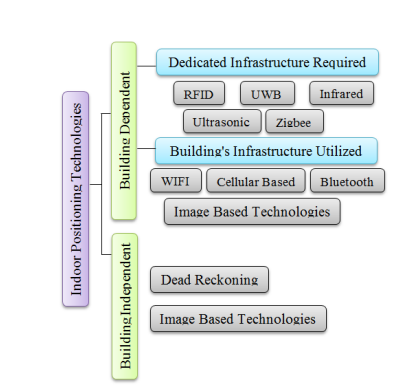
\includegraphics[scale=0.75]{classification_ips}
\caption{Classfication of indoor positioning technologies~\cite{ComparativeSurvey}}
\label{fig:ips_classification}
\end{figure}
\subsection{Location Information for Positioning Systems}
There are four commonly used types of information for \acrshort{ips}\cite{Liu2007}.
\begin{enumerate}
\item Absolute location: the location as a point inside a reference grid, shared across all objects used in the space.
\item Physical location: location displayed as a point in a coordinate system (x, y, z), either 2D or 3D.
\item Symbolic location: translates a physical location into a more human centred location name, e.g. office 213 on the 1st floor.
\item Relative location: location is based on the relative distance or proximity to a beacon or base point, e.g. rescue helicopter flying over sea trying to locate any survivors.
\end{enumerate}
\section{Distance Measurement Techniques}
\begin{figure}[h!]
\centering
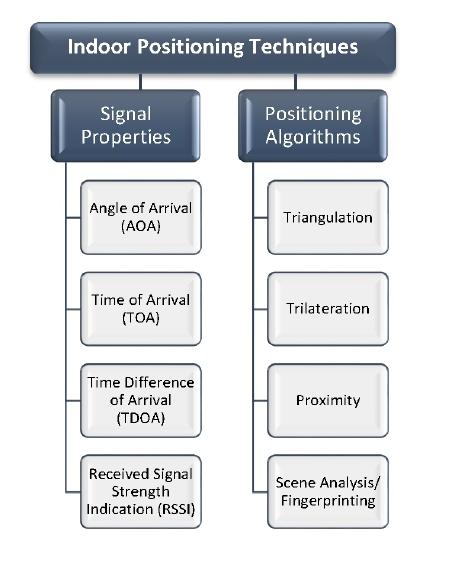
\includegraphics[scale=0.75]{classification_indoor_positioning_techniques}
\caption{Classification of indoor positioning techniques~\cite{Sakpere2017}}
\label{fig:ips_techniques}
\end{figure}
\subsection{Time of Arrival}
The \acrfull{toa} method is used to determine the distance between a \acrfull{tx} and \acrfull{rx}. In this method, the distance is calculated by the travelling time divided by the wave speed of the radio signal \cite{Loy2018}:
\begin{equation}
d = t * c
\end{equation}
Where d is the distance from \acrshort{tx} to \acrshort{rx} and c the constant speed of light (around $3.00 * 10^8 m/s$). This formula is based on research specifying the relationship between the propagation of a radio wave and its traversed range, which is a directly proportional relationship \cite{S2016}. Using the triangulation method for three available \acrlong{tx}s, the position of the \acrlong{rx} can be calculated. A synchronized clock is mandatory to provide accurate results, as the error rate is partially dependent on the speed of light, thus if there is an error of 1ms, the error in distance will be 300 meters. Hence the reason that \acrfull{gps} uses an atomic clock to ensure optimal accuracy \cite{Jindal}.
\begin{figure}[h!]
\centering
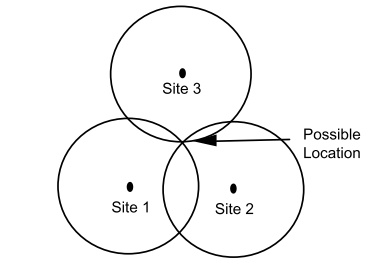
\includegraphics[scale=0.75]{toa}
\caption{Determining position in a two dimensional space by ~\acrlong{toa}~\cite{Jindal}}
\label{fig:toa}
\end{figure}
\subsection{Time Difference of Arrival}
\subsection{Angle of Arrival}
By using the \acrfull{aoa} method, the position of a device or \acrlong{mu} can be determined. This requires additional set up: directional antenna, thus \acrlong{tx}s. The intersection point of the lines indicating a direction signal resemble the possible location of the device, albeit without an exact error margin. The problem lies with the necessity of installing directional antenna arrays which contributes to higher cost than \acrlong{toa} and \acrlong{tdoa} \cite{Jindal}.
\begin{figure}[h!]
\centering
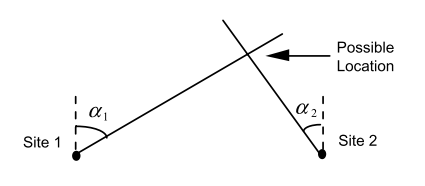
\includegraphics[scale=0.75]{aoa}
\caption{Determining position in a two dimensional space by ~\acrlong{aoa}~\cite{Jindal}}
\label{fig:aoa}
\end{figure}
\subsection{Received Signal Strength Indication}
\section{Indoor Positioning Techniques}
\subsection{Triangulation}
The angles of reference points are measured to calculate the position of the current position of the point, as visualized in \cite{fig:triang}. This method can only be used in combination with the distance method of \acrlong{aoa}.
\begin{figure}[h!]
\centering
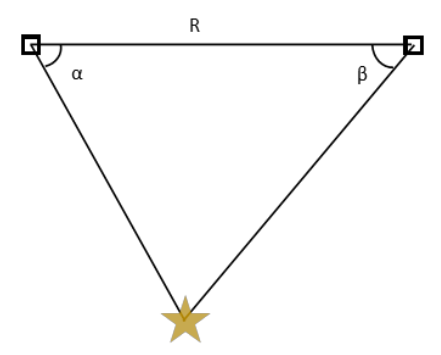
\includegraphics[scale=0.5]{triang}
\caption{Determining position using triangulation ~\cite{Loy2018}}
\label{fig:triang}
\end{figure}
\subsection{Trilateration}
\subsection{Scene Analysis/Fingerprinting}
\subsection{Proximity}
\section{Conclusion}
This thesis will cover the \acrshort{wlan} \acrlong{ips} technology and its implementation in a mobile application based on the provided project requirements.

\chapter{WLAN Indoor Positioning}
\section{Introduction}
One of the easiest \acrlong{ips} to implement are \acrshort{wlan} (specified by IEEE in their 802.11 specification) \acrshort{ips}s. The adoption of such a system comes without extra cost as most of the hardware is already prevalent in large, indoor environments.  The globally adopted operating bandwidth of \acrshort{wlan} is 2.4GHz (IEEE 802.11b, also known as Wi-Fi \cite{Li}), which does not come without its problems as discussed in a later section in this chapter \cite{Techopedia} \cite{ElectronicsNotes}\cite{Cisco}. In this chapter the most commonly used techniques to calculate the position of a \acrlong{mu} and the distance between a \acrlong{tx} and a \acrlong{rx}, being the \acrlong{mu}, are covered. After having covered the specific techniques, this chapter discusses the feasibility of this specific \acrlong{ips} with the complications of the 2.4GHz bandwidth as well as already commercially available systems.
\section{WLAN Characteristics}
\subsection{Signal Properties}
\subsection{Available Channels}
To minimize the chance of occurring interference, channels 1, 6 and 11 should be used for connecting devices. The WLAN channel width (of the 2.4GHz spectrum) is only 100MhHz wide, meaning channels 1, 6 and 11 are the only ones free of overlap \cite{Metageek}.
\begin{figure}[h!]
\centering
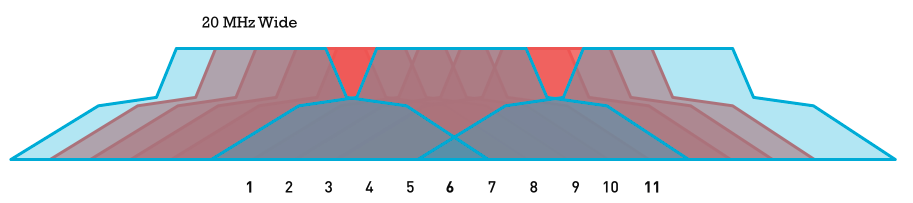
\includegraphics[scale=0.5]{wlan_channels}
\caption{Available WLAN channels in the 2.4~\acrshort{ghz} spectrum ~\cite{Metageek}}
\label{fig:ips_topologies}
\end{figure}
\subsection{Access Points}
\section{Indoor Positioning Topology}
Three topologies exists that can be used for gathering information about the position, as listed below \cite{Henniges2012}:
\begin{enumerate}
\item Network-based topology: position is determined by a central server and different \acrshort{ap}s;
\item Terminal-based: the position is identified by the mobile device;
\item Terminal-assisted: hybrid version of 1. and 2.
\end{enumerate}
\begin{figure}[h!]
\centering
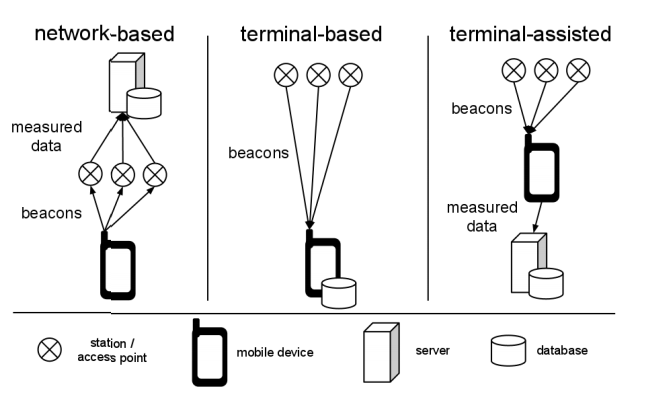
\includegraphics[scale=0.75]{ips_topologies}
\caption{IPS Topologies ~\cite{Henniges2012}}
\label{fig:ips_topologies}
\end{figure}
\subsection{Network-based}
This method only functions when the \acrshort{ap}s are adapted to not only receive network data but also signal data and redirect this to a central server that can handle and compute the data. This requires a change in the software of each \acrlong{ap}.
\subsection{Terminal-Based}
In this specific topology, the device driver of the \acrshort{ap} or terminal broadcasts beacons in its signalling range so a client can determine the best connectivity to a certain \acrshort{ap} and determine which \acrshort{ap} will be used. There are two ways of obtaining this information: 
\begin{enumerate}
\item active probing;
\item \acrshort{rf} monitoring
\end{enumerate}
RF monitoring is a form of passive scanning that listens to the periodic broadcasting by the \acrlong{ap}s, this is important to identify a connection in decline (due to significant noise on the signal, also known as \acrfull{snr}). When using active probing, the driver sends request frames to each known channel to detect any active WLAN connections. Each \acrshort{ap} receiving a request frame will in its turn respond with a response frame. These packets contain the \acrshort{mac} addresses of available devices. Based on this list of available devices and the corresponding signal strength (obtained from services that provide the information via the \acrshort{mac}-layer) an optimal \acrshort{ap} is selected\cite[p.~8]{Retscher}.
\subsection{Terminal-Assisted}
\section{Indoor Positioning Techniques}
The main difficulty in using this technique is determining the position of a device, relative to a Wi-Fi \acrfull{ap}. There are two mainly used technologies to determine the location of a \acrfull{mu}, being: positioning based on \acrshort{rssi} measurements (used in trilateration) and on empirical observations (fingerprinting) \cite{Frank2009}. Another less popular option is the proximity, presence or Cell of Origin technique that has less accuracy than the other two options.
\subsection{Proximity or Cell of Origin Technique}
This technique is not optimal to determine an absolute or relative position, however this technique is used when accuracy is not the most important factor. This method simply locates the \acrshort{ap} with the strongest \acrshort{rssi} value, which often is the closest to the \acrlong{mu}. This is an optimal technique to provide symbolic \acrlong{lbs} \cite{Sakpere2017}.
\begin{figure}[h!]
\centering
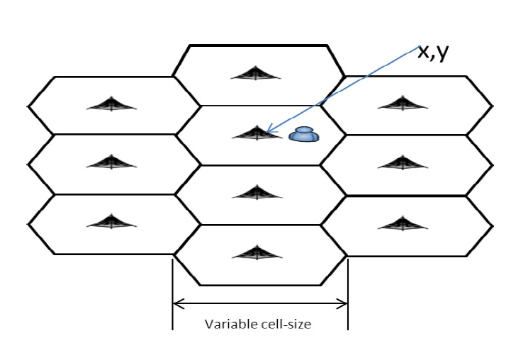
\includegraphics[scale=0.5]{coo}
\caption{Visual representation of the Cell of Origin technique ~\cite[p.12]{S2016}}
\label{fig:coo}
\end{figure}
\subparagraph{Conclusion} This technique is ideal when the accuracy is a less important factor and provides \acrlong{lbs} with a very low cost and fast response time.
\subsection{Trilateration Technique}
Trilateration, or multilateration, is based on a mathematical approach that incorporate the characteristics of the \acrshort{ap} and its signals, such are: characteristics of the radio signal (wavelength, frequency, noise etc.), \acrfull{mac} address of the \acrlong{ap} and the position of WLAN \acrshort{ap}s, without being limited to taking the signal strength in account. This approach requires three base points to calculate and determine a point in range of these three base points. Applying this method to the current case in which the available base points are the \acrshort{ap}s and the \acrshort{mu}, one has to calculate the distance of the \acrlong{mu} to each of the three \acrshort{ap}s in the vicinity. The main difficulty using this method is the estimation of the distances between both the \acrshort{ap}s and the device. Commonly used methods to determine the distance between both the AP as well as the mobile user include: \, \acrfull{toa} from transmitters or \acrfull{tdoa} \cite[p.~1]{Shchekotov} \cite[p.~60]{Mautz}.
\subsubsection{Geometric Principle}
As stated in the previous paragraph, trilateration requires an equation system containing three distance measurements between \acrshort{ap} and \acrlong{mu}. Using the euclidean distance between two points, this results in the following system or model \cite{CutTheKnot}:
\[ \sqrt{(x-x_1)^2 - (y-y_1)^2} = d_1 \]
\[ \sqrt{(x-x_1)^2 - (y-y_1)^2} = d_2 \]
\[ \sqrt{(x-x_1)^2 - (y-y_1)^2} = d_3 \]
By solving this system of equation, each distance is considered to be the radius of a circle, starting at the \acrshort{ap}. The three circles created by according radius contain an intersection point, the specific location of the user, as visualized in figure 4.1.
\begin{figure}[h!]
\centering
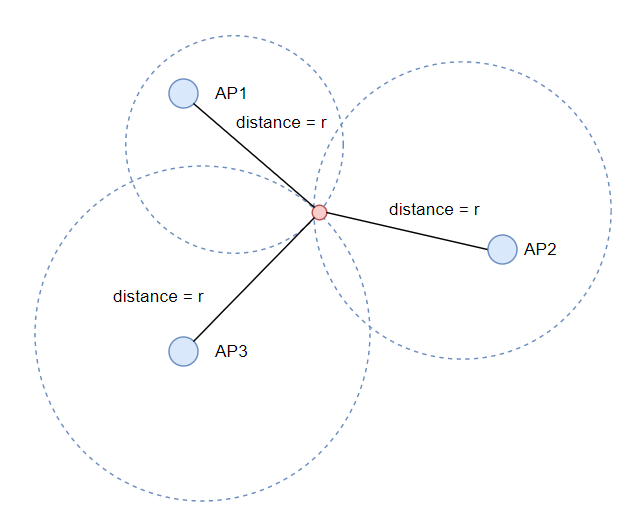
\includegraphics[scale=0.5]{euclidean_distance}
\caption{Euclidean distance resulting in geometric intersection of three circles, determining the position of a point in between these three points.}
\label{fig:euclidean}
\end{figure}
\subsection{Path Loss Positioning based on RSSI Measurements}
To handle the loss and gain of the radio signal, a free-space path loss model is used, as seen in an experiment in \cite[p.178]{Shchekotov}. Shchekotov's research is funded on the research of Sklar in 1997 that suggests that the average \acrshort{rssi} is distributed lognormally and can therefore be predicted by using a path loss model \cite[p.16]{S2016}. The path-loss model revolves around the calculation of the distance based on the attenuation of the signal \cite{Mautz}.
\begin{figure}[h!]
\centering
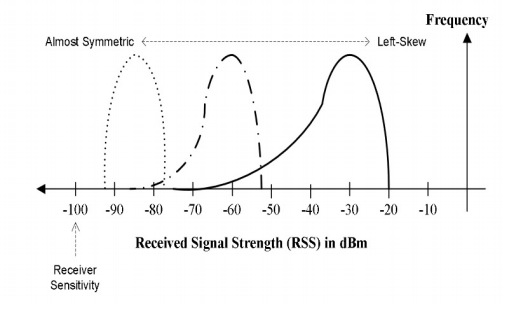
\includegraphics[scale=0.75]{distribution_of_rssi}
\caption{Distribution of ~\acrlong{rssi} ~\cite[p.16]{S2016}}
\label{fig:distribution_rssi}
\end{figure}
\begin{figure}[h!]
\centering
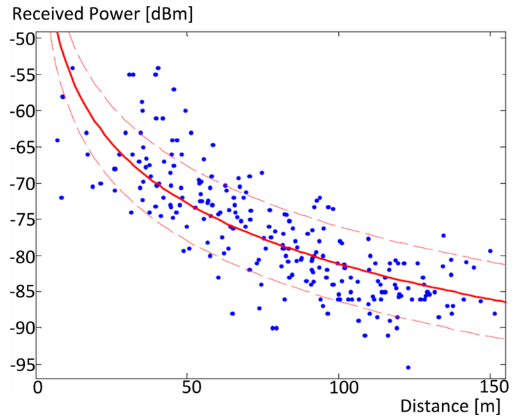
\includegraphics[scale=0.75]{rssi_distance}
\caption{Dependency of ~\acrlong{rssi} and distance ~\cite[p.61]{Mautz}}
\label{fig:rssi_distance}
\end{figure}
The empirical formula, solely based on measurements from the experiment so not a standard analytic model, provided by \cite{S2016} is as follows:
\[
FPSL = 20log10(d) + 20log10(f) - 27.55
\]
Where the \acrlong{tx}-\acrlong{rx} separation distance is annotated by the variable $d$ and the frequence in \acrfull{mhz} by $f$. $FPSL$ indicates the received signal strength path loss in \acrfull{dbm}. Based on the formula above and the one specified below, as specified in the research in \cite[p~13]{S2016} and \cite[p~6]{Wang2003}, the distance between a \acrlong{tx} and \acrlong{rx} can be calculated.
\[
P_r = P_t G_t G_r \frac{\lambda^2}{(4 \pi d)^2}
\]
In this formula, $G$ specifies gains of both \acrshort{tx} and \acrshort{rx} antennae, $\lambda$ specifies the wavelength, $d$ resembles the distance between the \acrlong{tx} and \acrlong{rx}
\subparagraph{Conclusion}
Based on the research done in \cite{Shchekotov}, the signal propagation model using a free-space path loss approach does not provide an accurate estimation of the user's current position due to fluctuations in the radio wave channel and decrease of accuracy with an increasing distance \cite[p~61]{Mautz} \cite[p~2]{Loy2018}. Nonetheless, this technique can be feasible in environments with less fluctuations and a denser distribution of \acrshort{ap}s, resulting in a smaller margin of error. 
\subsection{RSS Measurement Collection}
This method uses an empirical (observational) model, generated by trial runs using different calibration points with different \acrlong{ap}s. As seen in experiment in \cite{Shchekotov}, this experiments results in a table containing different measurements of different distances and the received signal strength in dBm, from \acrlong{tx} to the \acrlong{rx}. This empirical method results in a usable mathematical formula:
\[
\Delta = \sqrt{\sigma * t)^2 + A^2}
\]
In this equation $\Delta$ annotates the observational error in dBm, $\sigma$ is the standard deviation of the experiment, $t$ is the function of the t-distribution and $A$ is the observational error of the \acrfull{rx} ~\cite[p.178]{Shchekotov}. The error margin can be taken into account by applying this formula in a trilateration approach.
\begin{figure}[h!]
\centering
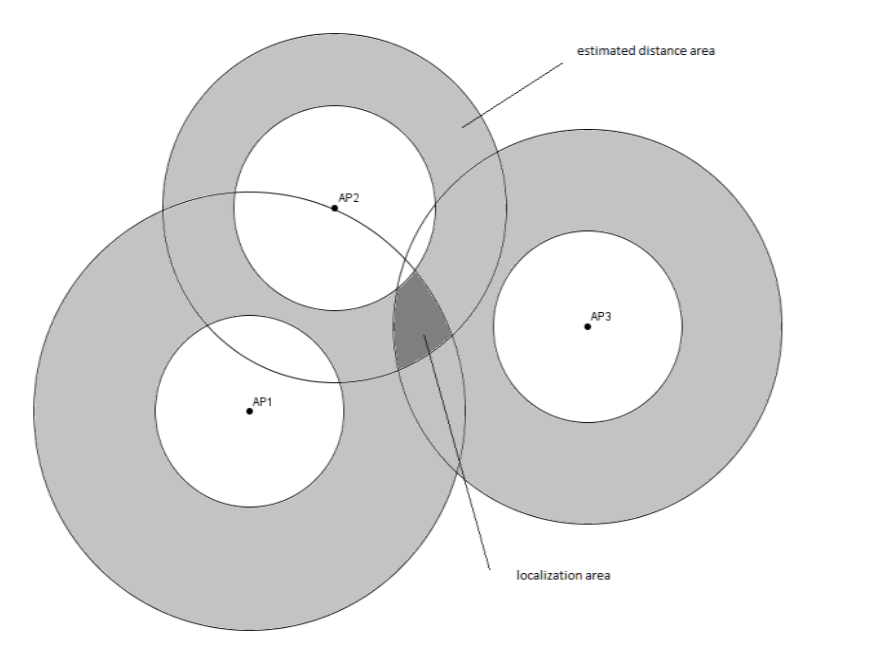
\includegraphics[scale=0.5]{estimated_distance_segments}
\caption{Estimated distance segments ~\cite[p.179]{Shchekotov}}
\label{fig:estimated_distance_segments}
\end{figure}
\subparagraph{Conclusion}
As seen in the trials performed in the research of \cite{Shchekotov}, this approach can be perceived as a special case of fingerprinting due to the creation of a \acrshort{rss} to \acrshort{ap} table. This method results in a more accurate estimation of the user's location by taking the error and deviation into account. However, this research was not based on extensive measurements and it is uncertain this approach will yield an optimal accuracy and precision.
\subsection{Fingerprinting Technique}
A computationally effective method of determining a user's location is the fingerprinting technique. This technique consists of two phases: offline acquisition of \acrshort{rssi} values at particular locations and an online phase with the actual implementation of periodically sent signals from a \acrshort{mu} \cite[p.~9]{Retscher}. This method bases itself only on the strength of the signal compared to trilateration that incorporates multiple methods to calculate the distance.
\begin{figure}[h!]
\centering
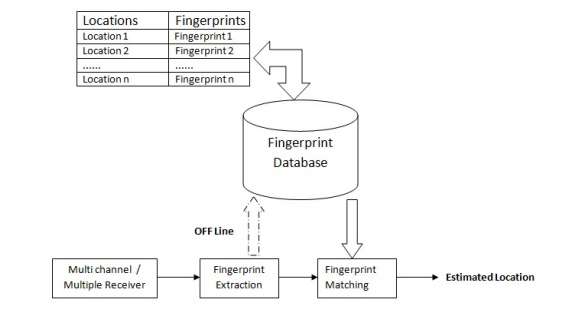
\includegraphics[scale=1]{fingerprint_chart}
\caption{Fingerprinting Stages ~\cite[p.11]{S2016}}
\label{fig:fingerprint_chart}
\end{figure}
\begin{figure}[h!]
\centering
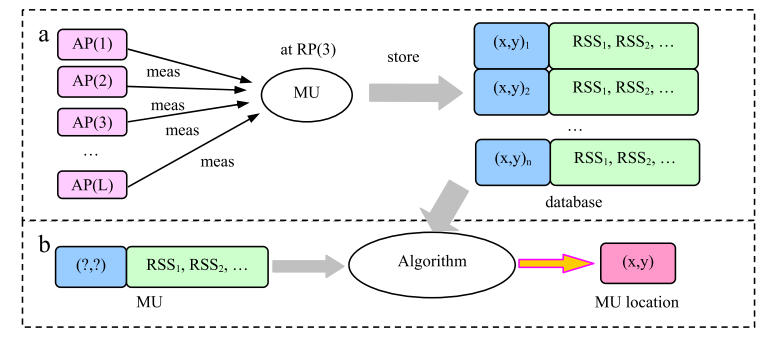
\includegraphics[scale=0.75]{fingerprinting_stages}
\caption{Fingerprinting Stages ~\cite[p.2]{Li}}
\label{fig:fingerprint_stages}
\end{figure}
\subsubsection{Offline Acquisition}
The offline stage of fingerprinting consists of defining and measuring calibration points, which is a major drawback as this is a time-consuming task. The result of the empirical measurements of different points is a radio map with signal strengths in relation to the specific points. The \acrshort{rssi} is measured a few times on each calibration points and afterwards stored inside a database. Each entry in the database is a fingerprint, f, with a corresponding ground-truth (\acrshort{rssi}), symbolized as a vector in a three dimensional vector space.
\subsubsection{Online Phase}
In the online phase, the fingerprints stored in the database are used to determine and estimate the current position of a \acrshort{mu}. The estimation of the distance is in most cases calculated using the Euclidean distance method as shown in \cite{fig:euclidean}. The most straightforward method is to determine the minimum distance between the observation (current position) and the \acrshort{ap}s in the vicinity. Another method is a probabilistic method that calculates the probability that the current \acrlong{rssi} measurements have the same position as a fingerprint corresponding in the fingerprint database \cite{Mautz}. This approach is based on the correlation values of the current observation and the fingerprints available in the database. This requires additional computing power but results in an increased accuracy.
\subsubsection{Improving Performance}
Contributing factors to increasing the performance, mainly accuracy and precision, are: number of \acrshort{ap}s per $m^2$, the amount of calibration points measurement in the offline phase, the density of those points and the fluctuations in  \acrshort{rssi} values.
\subparagraph{Conclusion}
This method requires a lot of time to set up the radio map in the offline phase, but results in a satisfactory accuracy, generally several meters, and precision. This is the preferred method of providing indoor location using a \acrshort{wlan}-based technology as it does not require additional equipment to be installed or configured. However, this technique is complex, hard to initially set up and does not scale well with an increase in users due to the increasing fluctuations in the radio signal that arise because of environmental factors, resulting in the need for re-calibrations at certain points in time with an increasing number of users.
\section{Feasibility}
\subsection{Security and Privacy}
\subsection{Cost}
\subsection{Performance}
\subsection{Environmental Effects on Radio Frequency and Fault Tolerance}
Radio frequency signals are subjected to interference from other signals. This included reflection, diffraction and scattering. These interferences on a radio frequency signal can result in a loss of accuracy and precision in an \acrlong{ips} and are therefore implications of this specific indoor positioning technology \cite{S2016}. 
\subsubsection{Indoor Environment}
Based on a study performed in \cite{Wang2003}, where the signal strength of a 2.4GHz radio wave was tested over a period of 24 hours, the signal strength contains some interferences but overall results in a mean signal strength of 47.17dBm. In \cite{fig:wang_test} the samples of the experiment are plotted in function of the time.
\begin{figure}[h!]
\centering
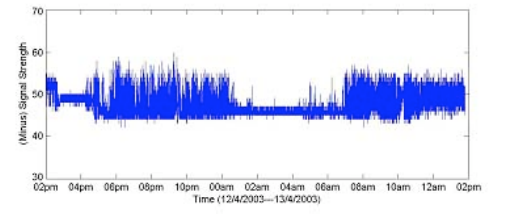
\includegraphics[scale=1]{wang_test}
\caption{24 hour static signal strength measurements ~\cite{Wang2003}}
\label{fig:wang_test}
\end{figure}
\subparagraph{Conclusion of experiment conducted in ~\cite{Wang2003}}
The experiment concludes that the radio signal of a WLAN infrastructure, operating on a 2.4GHz frequency, is stable and consistent, thus this signal can be used in calculations for positioning algorithms. However, the developer of such an algorithm needs to take the standard deviation into account as this differs throughout the use of different indoor environments, even on the level of floors, meaning that the signal strength on the first floor can differ on the third, based on environmental changes (e.g. moving persons, microwaves, other interfering electronic devices).
\subsubsection{SNR in WLAN}
The signal to noise ratio is the difference between the signal strength and the interfering signals. This is a factor to take into account when deploying any \acrshort{wlan} \acrlong{ips}. A satisfactory \acrlong{snr} should lie above 20 to 25 \cite{Hallock2015}.
\subsubsection{Signal Attenuation}
Signal attenuation, or signal loss, represents the loss of signal strength in \acrfull{db} of radio signals travelling through certain objects. The most common objects and their derived signal attenuation are represented below:
\begin{table}[]
\centering
\begin{tabular}{|l|l|}
\hline
\textbf{Object}             & \textbf{Signal Attenuation} \\ \hline
Plasterboard wall           & 3 dB                        \\ \hline
Glass wall with metal frame & 6 dB                        \\ \hline
Cinder block wall           & 4 dB                        \\ \hline
Office window               & 3 dB                        \\ \hline
Metal door                  & 6 dB                        \\ \hline
\end{tabular}
\caption{Objects with corresponding signal attenuation ~\cite[p.99]{Hallock2015}}
\end{table}
\subsubsection{Human Body}
The human body also has an effect on signals that are transmitted through the human body. As seen in the experiment by \cite{S2016} the difference of the standard deviation is 2.32dBm. The research conducted in \cite{Mautz} even reports a measurement error of nearly 15dBm.
This is why the fingerprinting technique is the favourable method to estimate the current position of a \acrlong{mu}, the fingerprinting provides a fault-tolerant method due to the multiple calibration measurements conducted in the offline phase, where the calibration should include signals passing through the human body.
\subsection{Complexity}
\subsection{Application Use}
\subsection{Commercial Availability}
\subsubsection{RADAR}
\subsubsection{COMPASS}
\subsubsection{Ekahau}
\section{Conclusion}

\chapter{Cisco CMX}
\section{Cisco CMX as IPS}
One of the companies that jumped on the bandwagon of the implementation of \acrlong{ips} is Cisco. Over the years they have developed a dashboard to gain intelligence from user's position such as hotspots where users gather most frequently and heat maps of different routes \acrlong{mu}s take. The definition provided by Cisco, states: ``Cisco’s CMX solution allows venues to simultaneously provide users with highly personalized content, provide services to customers to increase the customer experience, and gain visibility into customer behavior in their venues. CMX detects in-venue Wi-Fi enabled devices, prompts customers to connect to the wireless network, and engages them with value-added content and offers.`` \cite[p.~24]{Hallock2015}.
\subsection{Cisco MSE}
Cisco \acrfull{mse} is a platform that enables developers and users of this platform to centralize data, analyses and other \acrshort{wlan}-related statistics (e.g. coverage). Not only centralizing data but view the data is an important component of Cisco's \acrshort{mse}. Graphical plots such as heatmaps, interactive charts for user flows are part of this ecosystem (in CMX Analytics). It acts as the hardware engine behind the Cisco CMX technology, another option is to run the Cisco CMX platform on a dedicated server but to leverage all the possibilities of both CMX and MSE it is better to purchase the MSE appliance \cite{Shah}.
\section{CMX Services}
\subsection{CMX Cloud}
To leverage the latest cloud possibilities, Cisco developed a single cloud platform: DNA Spaces. This platform aims to centralize all location solutions into one single platform. It offers an improved experience for \acrlong{lbs} that are implemented using Cisco \acrshort{ap}s \cite{Ciscok} \cite{Cisco2019a}. DNA Spaces provides an \acrfull{api} that can be used to connect to other applications.
\subsection{CMX Connect}
\subsection{CMX Analytics}
\begin{figure}[h!]
\centering
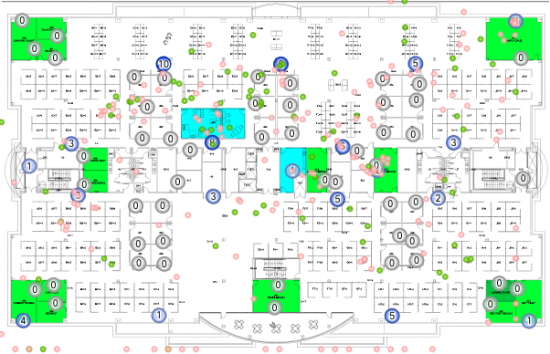
\includegraphics[scale=0.75]{cmx_map}
\caption{Positions of ~\acrlong{mu}s and which ~\acrlong{ap} they are connected to ~\cite{Shah2015a}}
\label{fig:toa}
\end{figure}
\subsection{CMX Engage}
\section{Location}
\subsection{Location Techniques}
\subsubsection{Proximity, Presence}
This technique is most feasible when dealing with outdoor positioning as it requires less \acrlong{ap}s but has less accuracy. According to the datasheet of Cisco \cite{Ciscoa}, the accuracy of this technique is limited to 10 to 30 metres. To calculate the user's position, the \acrshort{ap} with the strongest \acrlong{rssi} is picked as a correct representation of the \acrshort{mu}'s location.
\subsubsection{RSSI Triangulation}
\subsubsection{Hyperlocation}
\subsubsection{FastLocate}
\subsection{CMX Connect}
\subsection{CMX Analytics}
\section{Performance Metrics}
\subsection{Accuracy ~\& Precision}
\subsection{Coverage Area}
\subsection{Scalability}
According to documents provided by Cisco, most of the \acrshort{wlan} controllers are scalable with a decent throughput. Some statistics:
\begin{enumerate}
\item Cisco 5508: up to 500 \acrshort{ap}s and 7,000 clients are supported with a throughput of 8\acrfull{gbps}
\item Cisco 7510: up to 6,000 \acrshort{ap}s and 64,000 clients are supported with a throughput of 1\acrfull{gbps} in centrally switched traffic \footnote{All WLAN traffic is switched through a user-only WLAN network, meaning a locally switched WLAN can be active for employees without interfering with the user-only network. ~\cite{Woland}}
\end{enumerate}
There are numerous devices available that are not only dedicated to small or medium office, but also applicable to large multi-floor environments.
\subsection{Cost}
\subsection{Privacy}
\subsection{Conclusion}
\section{Conclusion}
\chapter{Integration using MapWize and IndoorLocation}
\section{IMplementation}
\chapter{Conclusion}
\input{chapters/conclusion}

\newpage
\printbibliography

\end{document}